%!TEX root = ../thesis.tex
%*******************************************************************************
%****************************** Third Chapter **********************************
%*******************************************************************************
\chapter{Neural tensor factorisation}

% **************************** Define Graphics Path **************************

\ifpdf
     \graphicspath{{Figs/Chapter3/}}
\else
    \graphicspath{{Chapter3/Figs/Vector/}{Chapter3/Figs/}}
\fi


Open domain question answering is concerned with reasoning about knowledge expressed in natural language. The Knowledge graphs (KG) framework has proved useful in encoding information about a domain that can be used for reasoning. The resource description framework (RDF) formalism, subject-predicate-object, is especially useful in representing dyadic relationships between entities expressed as KG nodes and edges. Link prediction can be used as a paradigm for solving the task of open domain question answering, where general questions can be posed as as potential relationships between nodes of a KG. Figure 3.1 shows how a KG can be used to answer a question like "In which country is the city of Cape Town?". 

\begin{figure}[H]
   	\centering
    	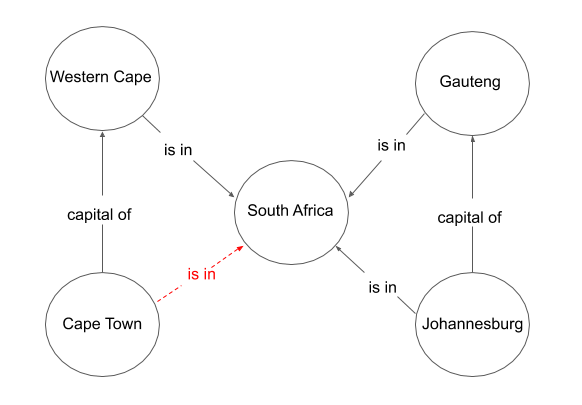
\includegraphics[width=0.5\textwidth]{Open_domain_question_answering_using_a_knowledge_graph.png}
	\caption{Open domain question answering using a knowledge graph.}
\end{figure}

\noindent The black edges indicate that the Cape Town is the capital of the Western Cape, and that the Western Cape is in South Africa. Similarly the capital of Gauteng is Johannesburg, and Johannesburg is in the same country as Gauteng. This information can be used to infer that Cape Town may also be in South Africa, indicated by the red edge. \par

\noindent Tensor factorisation has shown promise as a machine learning approach to temporal modeling of social networks, and in domains that are high-dimensional and sparse, such as singular value decomposition for recommender systems \unskip ~\citep{koren2009matrix}. Tensor factorisation is also compute efficient, and lends itself the GPU computation common in modern machine learning workloads. This approach decomposes entity-relational tensors into latent feature representations of entities and relations using an entity matrix and relational tensor respectively. The entity matrix is composed of entity vectors, and the relational tensor is composed of relational matrix slices which correspond to all the set of relation types in the KG, see figure 5. The product of the entity matrix, a relational matrix slice and transposed entity matrix is the bilinear tensor product. The operation generates an entity-relational tensor with unormalised scores of potential relationships between entities, indexed by relation. A probability of relation in the interval $ (0, 1) $ is then computed for each score using a sigmoid function. These probabilities are sorted in descending order to rank the plausibility of potential relationships. 

\begin{figure}[H]
	\parbox{.45\linewidth}{
   		\centering
    		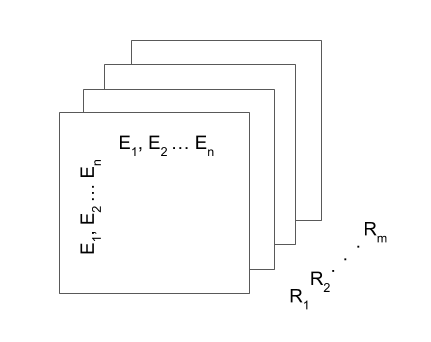
\includegraphics[width=0.4\textwidth, height=0.4\textwidth]{entity_relational_tensor.png}
		\caption{Entity relational tensor $ X $of size $ n \; x \; n $ with unnormalised relational scores.}
	}
	\hfill
	\parbox{.45\linewidth}{
   		\centering
    		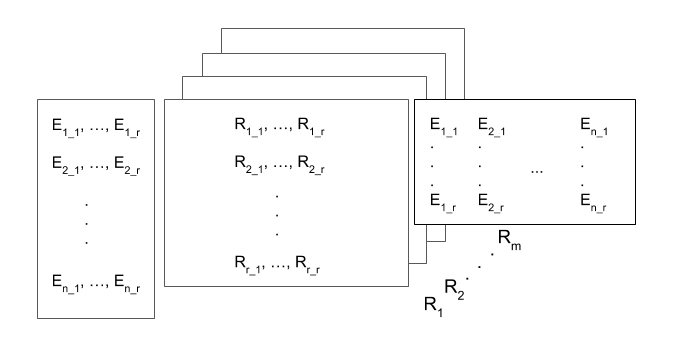
\includegraphics[width=0.45\textwidth, height=0.4\textwidth]{factorised_entity_relational_tensor_ARAt.png}
		\caption{Factorised entity relational tensor decomposed into entity matrix $ A $ of size $ n \; x \; r $, relational matrix $ R $ of size $ r \; x \; r $, and transposed entity matrix $ A^T $ of size $ r \; x \; n $.}
	}
\end{figure}

\noindent Previous latent feature approaches focused on limiting the total number of model parameters in order to scale to large knowledge bases (KBs), the representation of KG facts as RDF triples. This approach was often at the expense of complex entity-relational interaction modelling. The neural tensor network (NTN), a nonlinear extension of tensor factorisation, was the first successful link prediction technique to take advantage of the expressiveness of neural compositional models. It relies on adding a recursive network (RCN) \unskip ~\citep{pollack1990recursive} representation to the bilinear tensor product, and then using a fully connected layer to compute a relational score as a measure of confidence in a potential relationship between two entities. \par

\noindent Convolutional entity-relational modelling (ConvE) was similarly effective at extending tensor factorisation. ConvE concatenates a latent subject entity and relation vector into an entity-relational matrix, and then applies a 2-dimensional convolution operation on this matrix. A product is then taken between the generated representation and latent object entity to compute a relational score. Once again a sigmoid function is applied to produce a probability of relational plausibility between the two entities, indexed by relation. \par 

\noindent An alternative approach of applying convolution to neural tensor factorisation is the HypER model. HypER models entity-relational interactions by using a hypernetwork to generate 2-dimensional relation-specific convolutional filters. A 2-dimensional convolution is then taken between a latent subject entity and relational filter. Finally a product is taken between the generated entity-relational vector and a latent object entity, which computes a relational score. A sigmoid function is used to generate a probability of relational plausibility between the subject and object entity, indexed by relation. \par

\noindent In this chapter we assess the NTN model and attempt a simple improvement by applying adaptive moment estimation (Adam) optimisation and hyperparameter random search to the training algorithm. We then introduce HypER+, an extension of the HypER model which compensates for covariate shift introduced by hypernetwork generated relation-specific convolutional filters. Finally we extend HypER+ to make use of pre-trained GloVe word embeddings and attempt semantic enhancement of entities and relations. 


% **************************** First Section **************************

\section{Neural tensor networks}

\subsection{Neural tensor factorisation}
RESCAL introduced the bilinear tensor product for relational scoring \unskip ~\citep{nickel2011three}. This model makes use of entity vectors and a relational tensor, where each relation type is modelled as a matrix slice of the tensor. RESCAL is defined as follows:
\begin{equation}
	f_{i, j, k} = e_i^TW_ke_j = \sum_{a=1}^{H_e}\sum_{b=1}^{H_e}W_{a,b,k}e_{ia}e_{jb}
\end{equation}

\noindent where $f$ is the relational score, $e_i$ is the subject, $e_j$ is the object, and $W$ is the relational tensor. his is a linear model for entity-relational interactions that uses the dot product operator to construct a latent subject-relation representation, before computing a relational score using the dot product operator between the subject-relational representation and the object. RESCAL is thus a linear factorisation composition. \par

\noindent A natural extension to this method is to include a nonlinearity for entity-relational interaction modelling. This extension was introduced by Jenatton et al. \unskip ~\citep{jenatton2012latent}.Their model uses as sigmoid nonlinearity to compute a probability of relational plausibility from the relational score computed using the bilinear tensor product. The model is defined as follows:
\begin{subequations}
	\begin{gather}
		n_{i,j,k} = e_i^TW_ke_j \\
		\mathbb{P}\left [ R_j(S_i, O_k) = 1 \right ] = \sigma(n_{ik}^{j})
	\end{gather}
\end{subequations}

\noindent where $ n_{i,j,k} $ is the relational score, $ \sigma(t) = 1/(1 + e^{-t}) $ is the sigmoid function, a value in the range $\in \left ( 0, 1 \right ]$, and $\mathbb{P}$ is the probability of relational plausibility between $ S_i $ and $ O_k $ indexed by relation $ R_j $. This model introduces nonlinear entity-relational interaction to tensor factorisation. 

\subsection{Recursive neural tensor factorisation}

Socher and Chen et al.  \unskip ~\citep{socher2013reasoning} extend nonlinear tensor factorisation by introducing recursive entity representations in the composition of the relational score. Recursive networks (RCNs) try to capture the rules for word combinations by constructing compositional representations of two words \unskip ~\citep{socher2012semantic}. The NTN model tries to take advantage of these compositional rules by adding them to the bilinear tensor product and augmenting the nonlinear tensor factorisation. The RCN-extended nonlinear tensor factorisation model is defined as follows:
\begin{equation}
	g_{i,j,k} =  u_j^Tf(e_i^TW_j^{\left [1:m \right ]} e_k + V_j \left [ \begin{matrix} e_i \\ e_k \end{matrix} \right ] + b_j)
\end{equation}

\noindent where $g$ is the relational score, $f$ is the hyperbolic sigmoid function, $e_i^TW_j^{\left [1:m \right ]} e_k $ is the bilinear tensor product, $V_j \left [ \begin{matrix} e_i \\ e_k \end{matrix} \right ]$ is the recursive composition, a concatenation of the subject and object entity vectors, where a product is taken with a relational matrix $ V_j $ where rows correspond to respective relations, and $ b_j $ is the bias. \par

\begin{figure}[H]
   	\centering
    	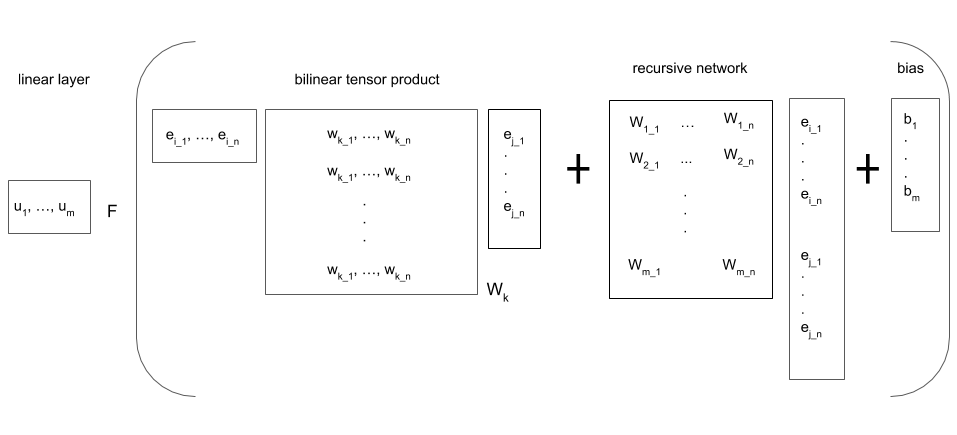
\includegraphics[width=0.5\textwidth, height=0.3\textwidth]{recursive_neural_tensor_network.png}
	\caption{Recursive neural tensor network.}
\end{figure}

\noindent The contrastive max-margin objective is minimised during training. This objective computes a confidence magnitude on a true correct sample (a fact present in the KB), and a confidence magnitude on a corrupt sample (a randomly generated fact not present in the KB). The correct and corrupt samples are used by the objective as follows:
\begin{equation}
	J(\si{\ohm}) =  \sum_{i=1}^N \sum_{c=1}^C \max(0,1 - g(T^{(i)}) + g(T_c^{(i)})) + \lambda \left \lVert \si{\ohm} \right \rVert_2^2
\end{equation}

\noindent where $J$ is the loss value, $\si{\ohm}$ are the model trainable parameters $u, W, V, b $, and $ E $. $N$ is the number of training triplets, $C$ is the number of randomly corrupted facts. $ g(T^{(i)}) $ is the confidence in the true fact computed by the model, and $ g(T_c^{(i)}) $ is the confidence in the corrupt fact computed by the model. Finally $\lambda\left\lVert \si{\ohm} \right\rVert_2^2$ is the ridge ($L_2$) regression regulariser. \par

\noindent The NTN model training algorithm also makes use of pre-trained word vectors developed by Turian et al. \unskip ~\citep{turian2010word}. These are 100-dimensional embeddings, which are aggregated from the set of words that represent an entity. For example for the entity \textit{homo sapiens}, the resulting word representation is $V_{homo \; sapiens} = 0.5(V_{homo} + V_{sapiens})$. These word vectors are trainable, and updated using backpropagation, to produce a distributed word representation that aligns with the KB. \par

\noindent \textbf{Modern optimisation.} Deep model training can suffer from noisy gradient signals when using stochastic gradient descent, mini batch optimisation and regularisation techniques such as dropout. Deep models can also suffer from insufficient signal to update parameters, a problem known as sparse gradients. Adaptive moment estimation (Adam) is a first order gradient-based stochastic optimisation algorithm that compensates for this noise \unskip ~\citep{kingma2014adam}. It computes the adaptive learning rates for parameters using the first and second order moments of the gradient, combining the advantages of AdaGrad ~\citep{duchi2011adaptive} and RMSprop ~\citep{tieleman2012lecture}. Adam efficiently regulates the size of parameter updates, accelerating toward local optima and remaining small in regions with a small gradient signal, sparse regions. \par

\noindent Setting model hyperparameters remains a challenge in deep model training. A simple method proposed to address this problem is hyperparameter random search \unskip ~\citep{bergstra2012random}. This approach improves on grid search by matching or exceeding model performance in a fraction of the compute time. It takes advantage of the fact that for most datasets only a subset of the hyperparameters contribute meaningful variance in model performance, eliminating the need for an exhaustive brute force search over a large combinatorial search space. \par

\noindent \textbf{Training algorithm.} Doss et al. reimplement the NTN model in TensorFlow \unskip ~\citep{abadi2016tensorflow}. This model severely underperforms compared to the original model, relying on AdaGrad optmisation and the same hyperparameters. We apply Adam optimsation as well as hyperparameter random search, in an attempt to improve its performance. The new training algorithm is as follows: 

\medskip

\begin{algorithm}[H]
	\For{Epoch}{ // repeat for $N$ experiments using random uniform hyperparameter configuration \\
		\SetAlgoLined
		\textbf{Input} 
		Training set \begin{math} D = \{(x_i, y_i)\}_{i=1}^N \end{math}, of samples and labels\;
  		\begin{math} S_{batch} \gets sample(S, b) \end{math} // sample a minibatch of size \begin{math} b \end{math} \\
	 	\For{(x, y) \begin{math} \in S_{batch} \end{math}}{
     			\begin{math} y^{'}_{correct} \gets predict(x) \end{math} // predict label for sample \\
			\begin{math} y^{'}_{corrupt} \gets predict(x) \end{math} // predict label for sample \\
			\begin{math} e \gets contrast(y_{correct}, \; y_{corrupt}, \; y^{'}_{correct}, \;  y^{'}_{corrupt}) \end{math} // compute error
     		}
		Update model w.r.t. \begin{math}  e \end{math} // using Adam optimser \\
	}
	\caption{Updated NTN training algorithm}
\end{algorithm} 

\newpage


% **************************** Second Section **************************

\section{Hypernetwork tensor factorisation}

\subsection{Convolutional factorisation}

ConvE introduced the convolutional operator to neural tensor factorisation \unskip ~\citep{dettmers2018convolutional}. Specifically, this operator increases expressiveness in entity-relation interaction modelling by using 2-dimensional convolutions, which are particularly effective at modelling the interactions of entities involved in a large number of relations. ConvE concatenates subject and predicate matrices along the row axis, creating a 2-dimensional entity-relational matrix. Convolutional filters are then applied to this representation, producing feature maps which are flattened by a fully connected layer. The dot product of this generated representation is then taken with the object vector, computing an unnormalised relational score between the subject and object, before a sigmoid function is applied to produce a probability of relational plausibility. The model is defined as follows:
\begin{equation}
	\psi_r(e_s, \; e_o) = g(vec(f(\left [ \overline{e_s}; \; \overline{r_r} \right ]*w))W)e_o
\end{equation}

\noindent where $ \psi_r $ is the relational score, $ e_s $ is the subject, $ e_o $ is the object, and $ r $ is the predicate. $ f $ is the concatenation operation between the subject and predicate, $ w $ contains the 2-dimensional convolutional filters, and $ * $ is the convolutional operator. $ vec $ reshapes the feature map tensor into a vector which is passed through a fully connected layer parameterised by $ W $, and then $ g $, a ReLU nonlinearity. ConvE is thus a convolutional tensor factorisation. 

\begin{figure}[H]
   	\centering
    	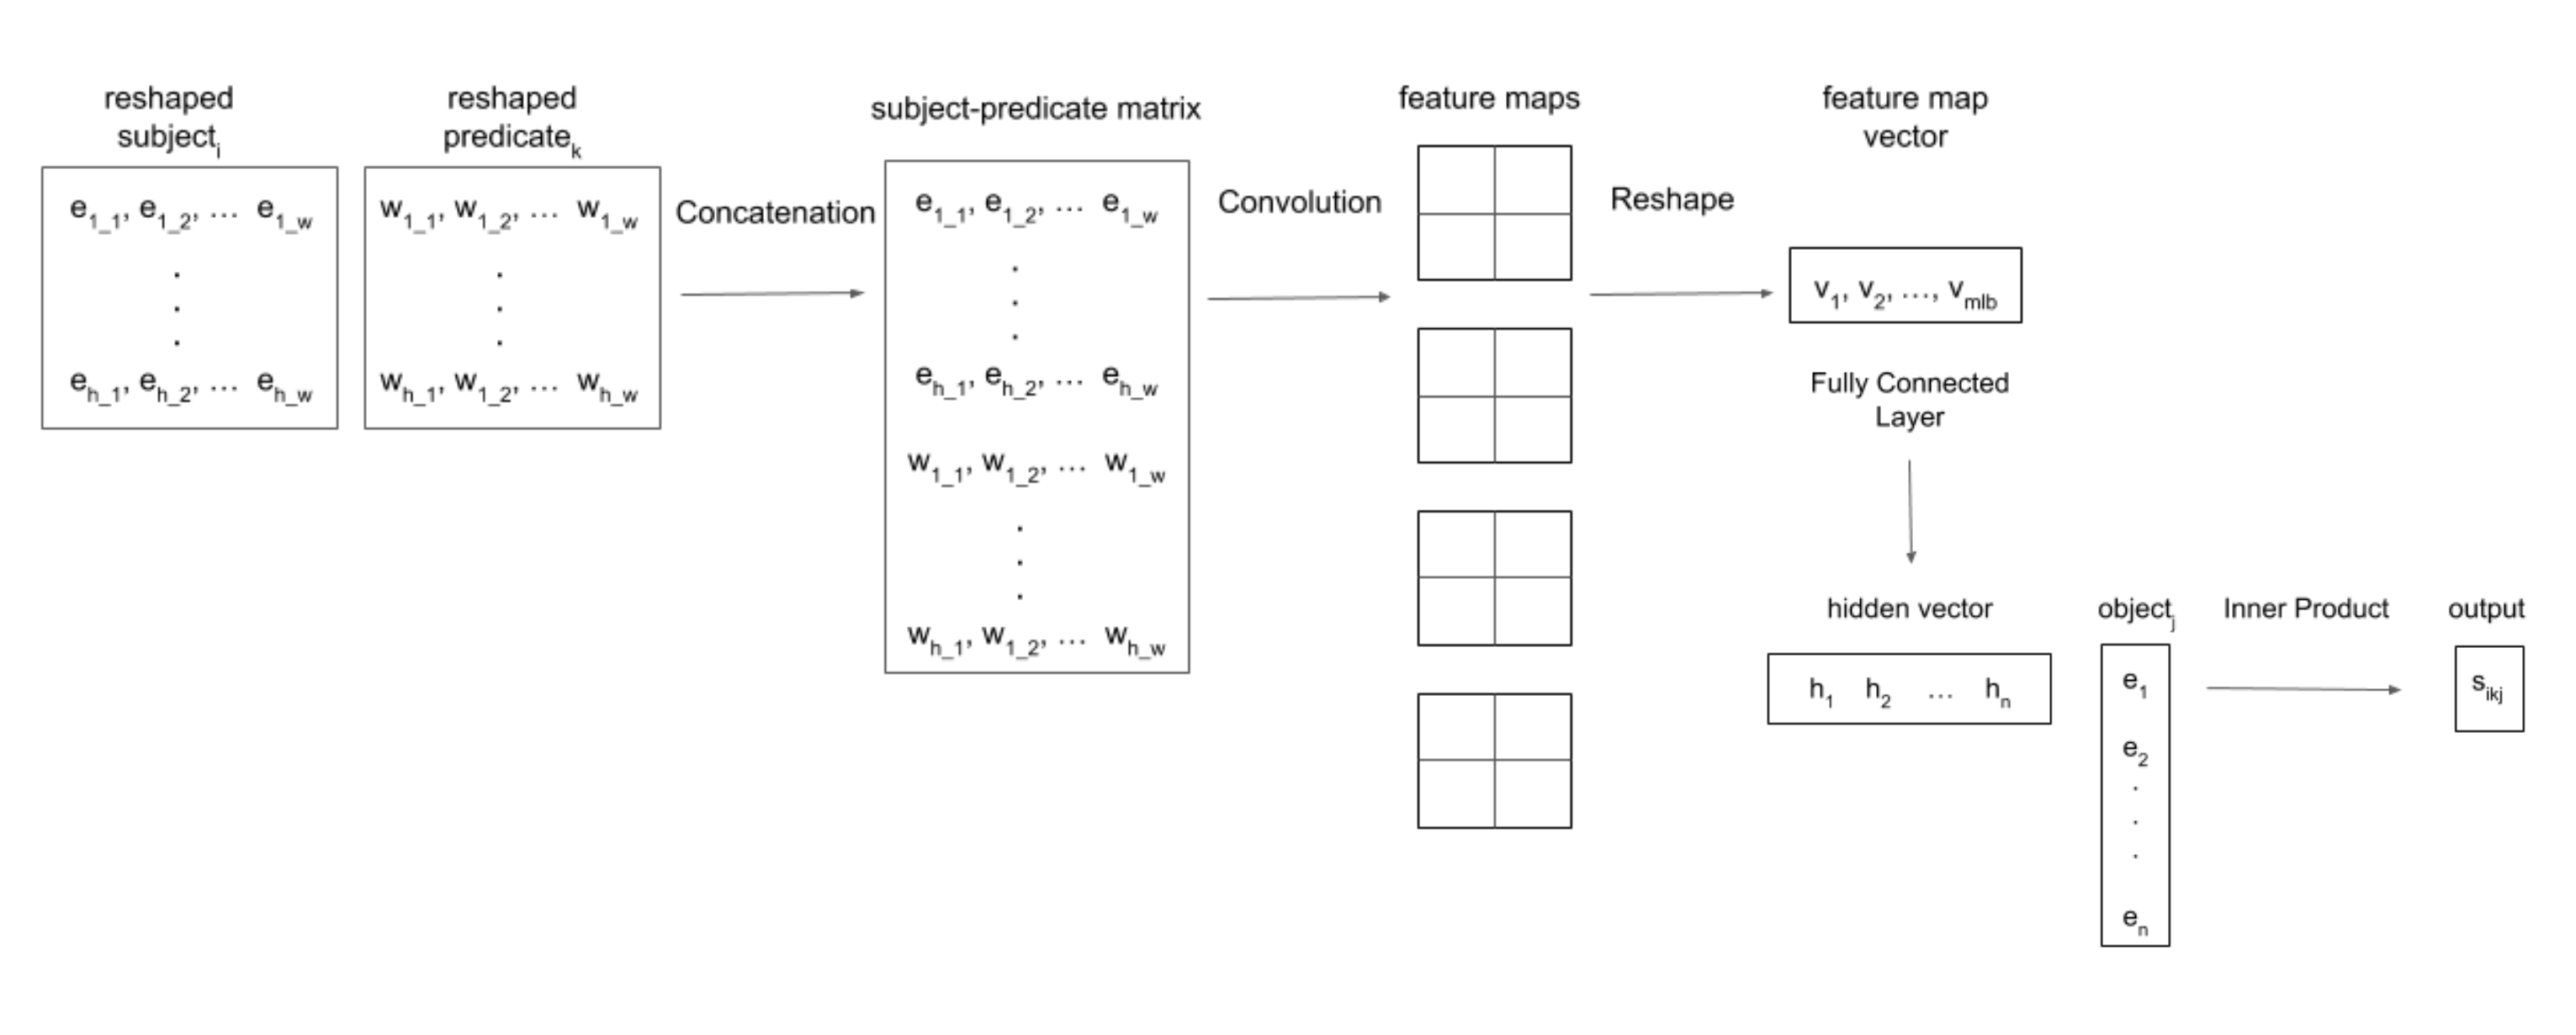
\includegraphics[width=0.7\textwidth, height=0.4\textwidth]{convolutional_entity_representations_final}
	\caption{Convolutional entity representations.}
\end{figure}

\newpage

\noindent The computed relational probability is defined as follows: 
\begin{equation}
	\mathbb{P} = \sigma(\psi_r(e_s, \; e_o)) 
\end{equation}

\noindent The binary cross-entropy objective is minimised during training. This objective is particularly effective as we expect only a single true class (a single object from the set of all entities) during inference, modelled as $1$, and every other class to be false, $0$. The objective is defined as follows:
\begin{equation}
	L(p, \; t) =  -\frac{1}{N}\sum_i(t_i \cdot log(p_i) + (1 - t_i) \cdot log(1 - p_i))
\end{equation}

\noindent where $ L $ is the loss value, $ p_i $ is the relational probability computed by the model, and $ t_i $ is the target. $ N $ is the batch size, and $ i $ is the sample index.

\subsection{Hypernetwork factorisation}

Hypernetworks are meta networks that generate parameters for a main network \unskip ~\citep{ha2016hypernetworks}. The networks essentially index the parameters of a main network as a configuration given input. This input is typically in the form of an embedding vector that describes all the weights of a given layer. The configuration is learned given a scenario experienced by the main network, for example when performing sequence prediction it may be advantageous for the main network to change its behaviour (parameter configuration) depending on the sequence window. The hypernetwork model can be defined as follows: 
\begin{equation}
	K_j = g(z_j), \quad \forall j = 1, \dots, D
\end{equation}

\noindent where $ K_j $ contains the parameters of layer $ j $, $ g $ is the hypernetwork composition, and $ z_j $ is the hypernetwork input. \par

\noindent HypER is inspired by ConvE, and implements a convolutional operator that models entity-relational interactions \unskip ~\citep{balazevic2019hypernetwork}. It makes use of a hypernetwork to generate relation-specific convolutional filters. The subject and relational filter are then used in a convolution operation to generate latent representations which are flattened by a fully connected layer. The dot product of this generated representation is then taken with the object vector, producing a measure of confidence in the relation, before a logistic sigmoid is applied to compute a probability of plausibility. The model is defined as follows: \newpage

\begin{equation}
	\phi_r(e_s, \; e_o) = f(vec(e_s * (vec^{-1}(w_rH)))W)e_o
\end{equation}

\noindent where $ \phi_r $ is the relational score, $ e_s $ is the subject, and $ e_o $ is the object. $ w_r $ is the predicate input and $ H $ is the parameterised matrix of the fully connected layer of the hypernetwork, $ vec^{-1} $ is the transformation that reshapes the output of the hypernetwork into a set of relation-specific convolutional filters. $ * $ is the convolutional operator, $ vec $ reshapes the feature map tensor into a vector which is passed through a fully connected layer parameterised by $ W $, and then $ f $, a ReLU nonlinearity. HypER is thus a hypernetwork convolutional tensor factorisation. 

\begin{figure}[H]
   	\centering
    	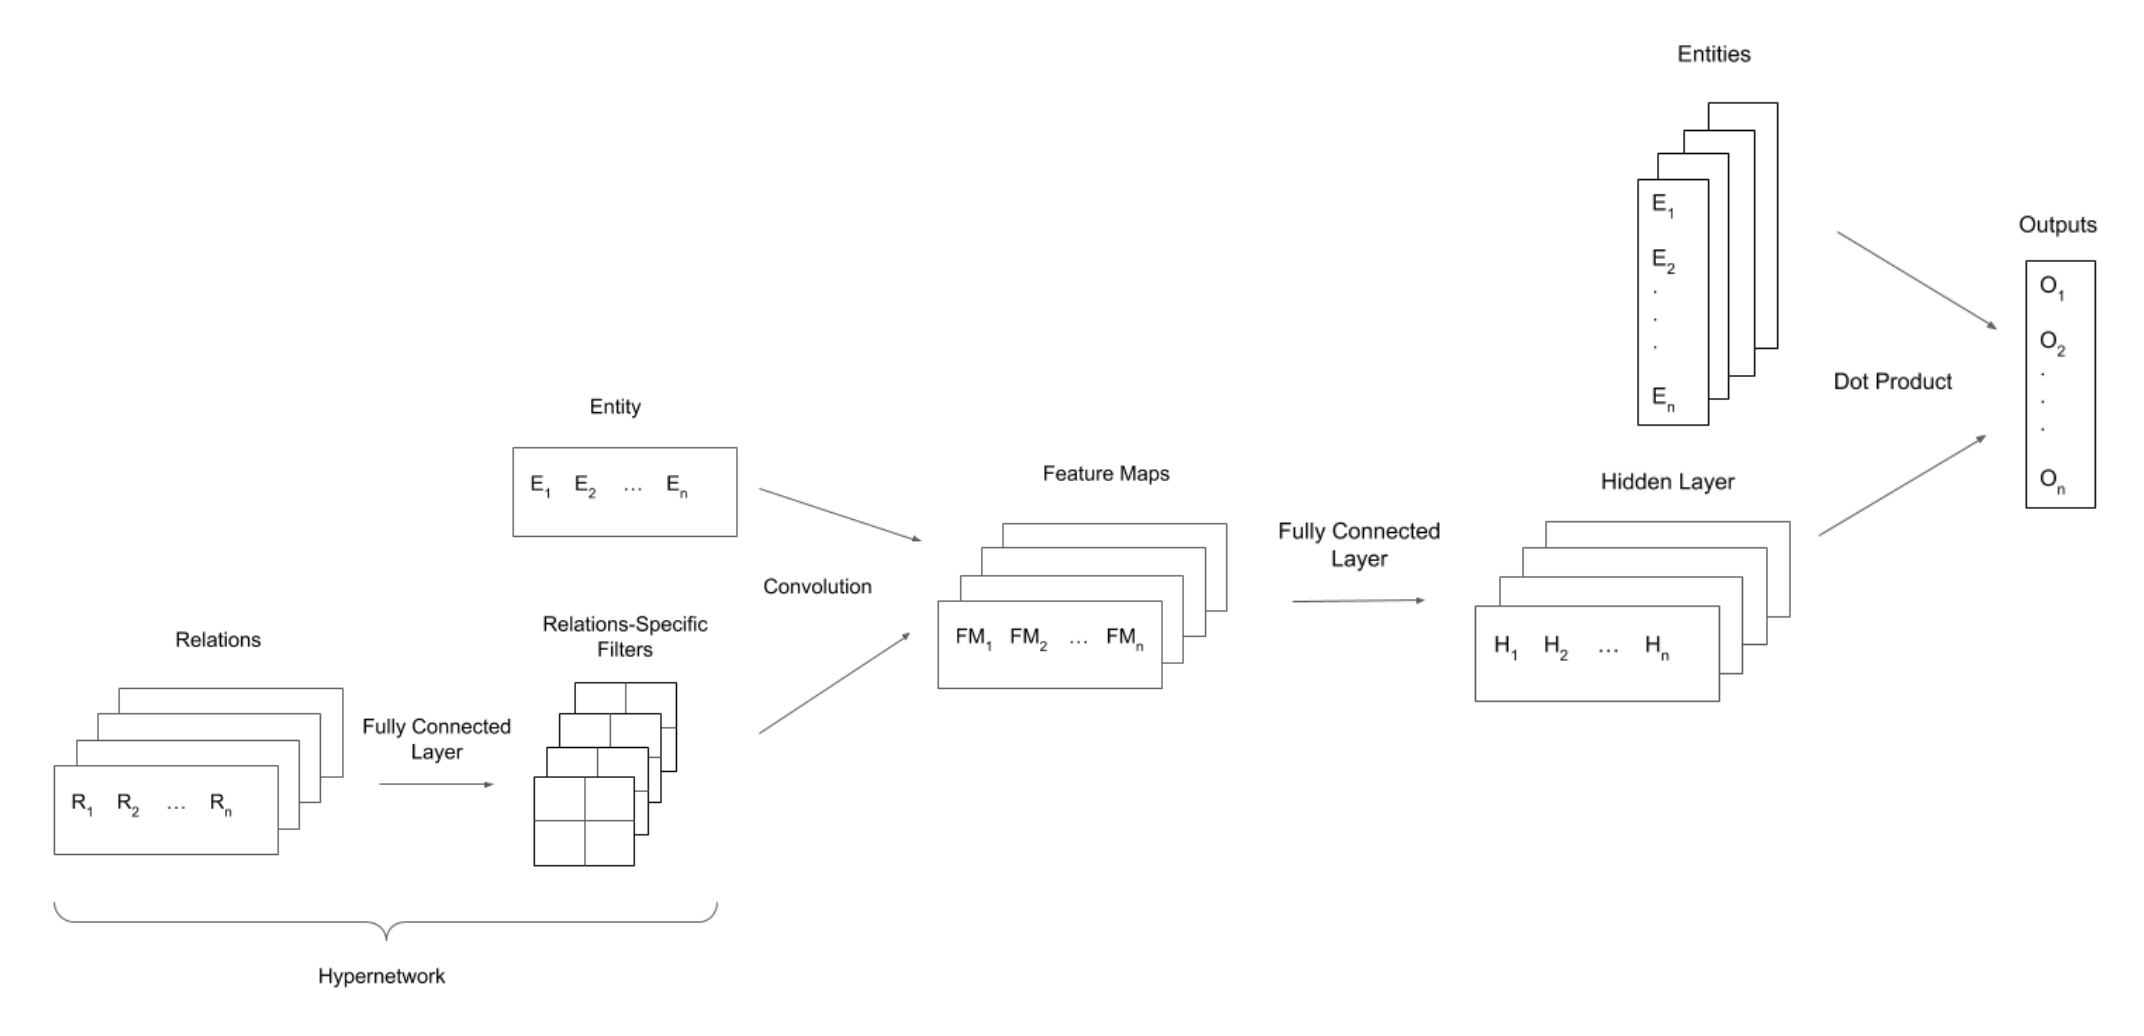
\includegraphics[width=0.7\textwidth, height=0.5\textwidth]{hyper_neural_tensor_network_final}
	\caption{Hypernetwork convolutional entity representations.}
\end{figure}

\noindent The computed relational probability is defined as follows: 
\begin{equation}
	\mathbb{P} = \sigma(\phi_r(e_s, \; e_o)) 
\end{equation}

\noindent The HypER training algorithm minimises the binary cross-entropy objective. HypER entities and relations are intialised using Xavier initialisation \unskip ~\citep{glorot2010understanding}, drawn from a distribution with zero mean and finite variance. \par

\noindent \textbf{Hyper covariate shift}. We make the observation that hypernetworks may also suffer from covariate shift. The network parameters are adjusted during training, resulting in a distributional drift across the entire main network as training progresses. To address this problem, we introduce batch normalisation between the hypernetwork and main network. We adjust the model accordingly, and introduce HypER+. \par

\noindent \textbf{Training algorithm}. HypER+ is trained using the binary cross-entropy objective. We use the same hyperparameters as the original HypER model, as well as the Adam optimiser. The HypER+ training algorithm is as follows: 

\medskip

\begin{algorithm}[H]
	\SetAlgoLined
	\textbf{Input} 
	Training set \begin{math} D = \{(x_i, y_i)\}_{i=1}^N \end{math}, samples and labels\;
  	\begin{math} S_{batch} \gets sample(S, b) \end{math} // sample a minibatch of size \begin{math} b \end{math} \\
	 \For{(x, y) \begin{math} \in S_{batch} \end{math}}{
     		\begin{math} y' \gets predict(x, \; y') \end{math} // predict label for sample \\
		\begin{math} e \gets y' - y \end{math} // compute error
     		}
	Update model w.r.t. \begin{math}  e \end{math} // using Adam optimser \\
	\caption{HypER+ Training Algorithm}
\end{algorithm} \bigskip
 
\noindent \textbf{Pre-trained word vectors}. We then apply pre-trained GloVe word vectors \unskip ~\citep{pennington2014glove} to the HypER+ training algorithm. We use these word vectors to initialise  200-dimensional embeddings, which are aggregated by the set of words that represent an entity or relation, the same method of aggregation used for pre-trained word vectors used during NTN training. Similarly, these word vectors are trainable, and updated using backpropagation.  


%********************************** %Third Section  **************************************

\section{Summary}

In this chapter we've discussed: \newline
\textbf{Neural Tensor Networks.} An early successful attempt at using the expressive power of neural networks for link prediction. This model also makes use of RCNs, which try to model semantic compositionality, and this model makes use of pre-trained word vectors to improve link prediction performance. We apply modern stochastic and hyperparameter optimsiation techniques to the NTN training algorithm, namely Adam and hyperparameter random search. \newpage
\textbf{Hypernetwork Tensor Factorisation.}  Hypernetworks can be used to generate parameters for other networks. This approach has the effect of applying a configuration to a neural network, and changing its behaviour given indexing input. A hypernetworks were used to generate parameters for a convolutional network in the model HypER. Concretely, HypER generates relation-specific convolutional filters which are used in a neural factorisation approach to link prediction. We adjust HypER to compensate for the covariate shift caused by the hypernetwork and introduce HypER+. We then extend HypER+ to make use of GloVe pre-trained word vectors by initialising entities and relations using these embeddings. \newline
